\section*{Question 3 --- Non-isothermal CSTR}
\answer{(a) State-space model}
Define $\nu=q/V$, $\beta=-\Delta H/(\rho C_p)$, $\gamma=UA/(\rho C_pV)$ and $\kappa(T)=k_0e^{-E/(R_gT)}$, with all rates expressed in seconds. For $x_1=C_A$, $x_2=T$, input $u=T_c$ and output $y=T$,
\begin{equation}
x=\begin{bmatrix}C_A\\T\end{bmatrix},\qquad
\boxed{\dot x=
\begin{bmatrix}\nu(C_{Af}-x_1)-\kappa(x_2)x_1\\\nu(T_f-x_2)+\beta\kappa(x_2)x_1-\gamma x_2\end{bmatrix}
+\begin{bmatrix}0\\\gamma\end{bmatrix}u},\qquad
y=\begin{bmatrix}0&1\end{bmatrix}x.
\end{equation}
The plant integrates concentration and temperature separately (Appendix~A).

\answer{(b) Linearization, validity and zero dynamics}
The input appears after one output derivative:
\begin{equation}
\dot y=\nu(T_f-T)+\beta\kappa(T)C_A+\gamma(u-T).
\end{equation}
Choose
\begin{equation}
\boxed{u=T+\frac{v-\nu(T_f-T)-\beta\kappa(T)C_A}{\gamma}}
\quad\Longrightarrow\quad\dot y=v.
\end{equation}
The new coordinates $z_1=T$, $\eta=C_A$ satisfy
\begin{equation}
\dot z_1=v,\qquad \dot\eta=\nu C_{Af}-[\nu+\kappa(z_1)]\eta.
\end{equation}
The relative degree is $1<2$, leaving one internal state. The coordinate change is an invertible permutation. For $\gamma\ne0$, the law is defined for $T>0$, $C_A\ge0$; practical operation also requires an achievable coolant temperature.

Set the shifted output $T-T_d$ to zero, so that $T\equiv T_d$. The zero dynamics are
\begin{equation}
\dot\eta=\nu C_{Af}-[\nu+\kappa(T_d)]\eta,\quad
\eta^*=\frac{\nu C_{Af}}{\nu+\kappa(T_d)},\quad
\eta(t)=\eta^*+[\eta(0)-\eta^*]e^{-[\nu+\kappa(T_d)]t}.
\end{equation}
For $\nu>0$ and $\kappa(T_d)\ge0$, the internal equilibrium is asymptotically stable; the reactor is minimum phase in this domain.

\answer{(c) Implementation}
The linearizing law receives $C_A$, $T$ and virtual temperature rate $v$, and commands $T_c$. Both states are fed back; the original nonlinear balances are retained.

\answer{(d) Temperature tracking with 5 s settling}
For constant $T_d$, choose $v=\lambda(T_d-T)$. Then $\dot e=-\lambda e$ and $e(t)=e(0)e^{-\lambda t}$, giving
\begin{equation}
\boxed{\lambda=\frac{-\ln\varepsilon}{T_s}},\qquad
\varepsilon=0.02,\ T_s=5\ \mathrm{s}
\quad\Longrightarrow\quad\lambda=0.782405\ \mathrm{s}^{-1}.
\end{equation}
For simulation, $\nu=\gamma=1/60$ s$^{-1}$, $k_0=7.2\times10^{10}/60$ s$^{-1}$, $E/R_g=8750$ K, $\beta=200$ K\,L/mol, $C_{Af}=1$ mol/L and $T_f=350$ K. At $T_d=330$ K, $\eta^*=0.819833$ mol/L and the internal time constant is $[\nu+\kappa(T_d)]^{-1}=49.19$ s. Initially $T=310$ K and $C_A=\nu C_{Af}/[\nu+\kappa(310)]=0.961796$ mol/L. The reference changes to 330 K at 1 s. Simulate 180 s using \texttt{ode45}, maximum step 0.02 s and relative/absolute tolerances $10^{-8}/10^{-10}$.
\begin{center}
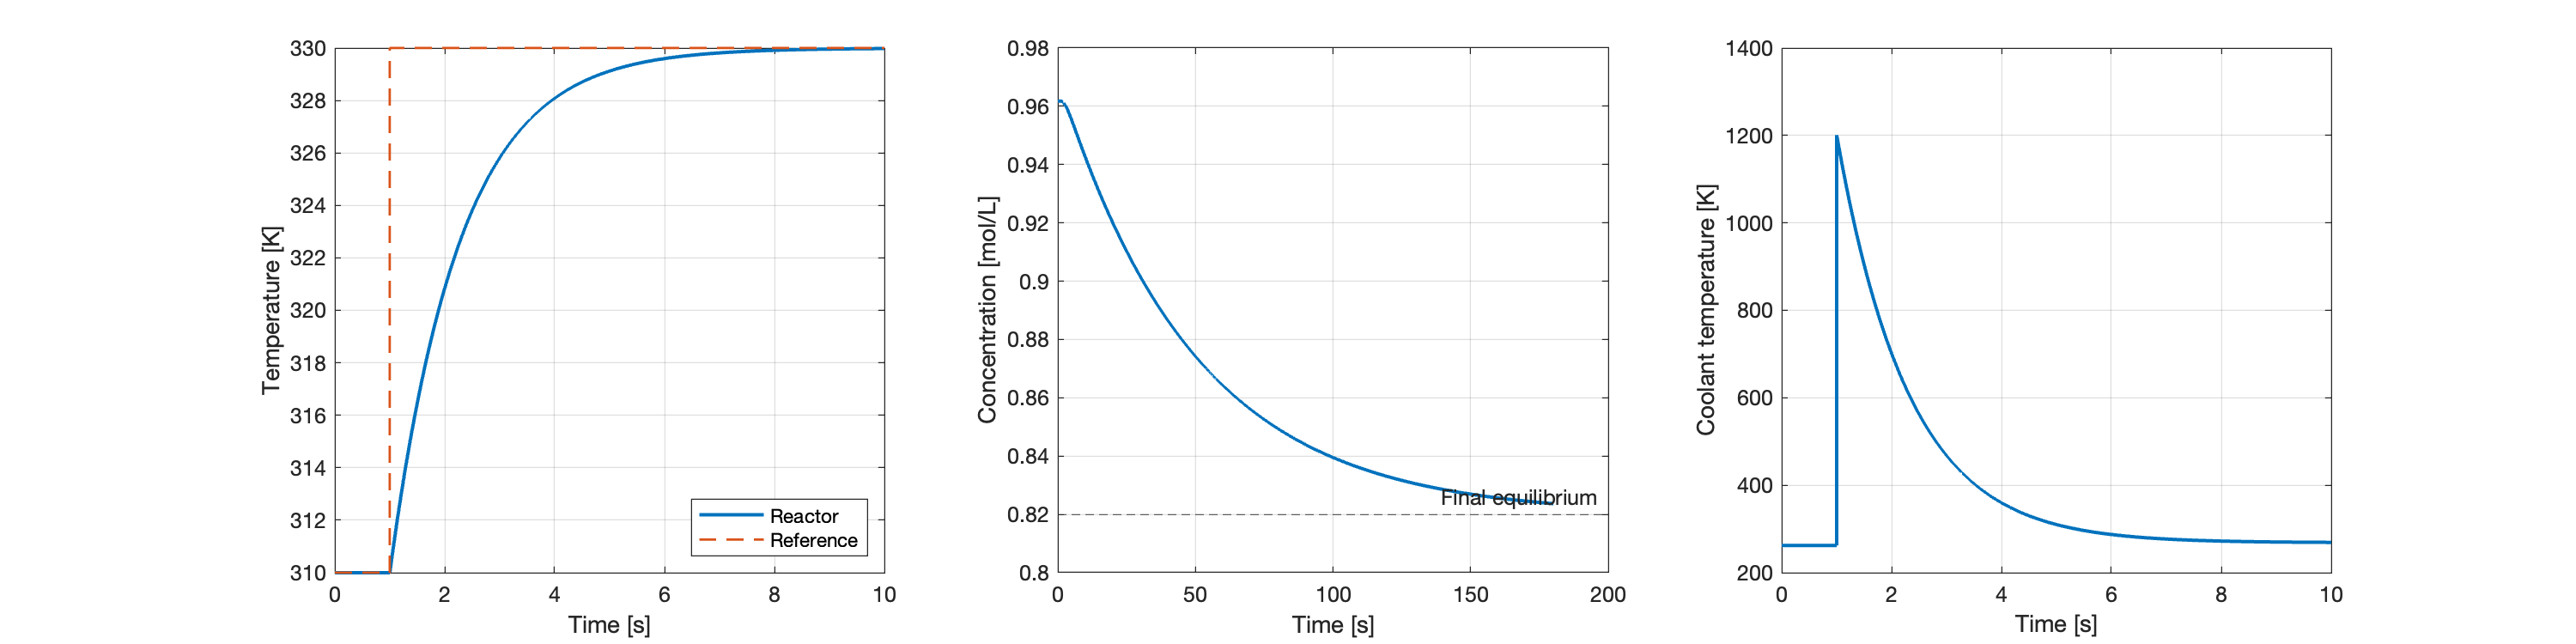
\includegraphics[width=0.95\linewidth]{report_cstr_response.png}
\reportcaption{Simulated temperature tracking, concentration and coolant command. Temperature and concentration use different time scales.}
\end{center}
The temperature follows $T(t)=330-20e^{-\lambda(t-1)}$ K for $t\ge1$ s, without overshoot. The sampled 2\% settling time is \textbf{5.02 s}, consistent with the 5 s target and 0.02 s sampling interval. Concentration reaches 0.82370 mol/L at 180 s and converges toward 0.819833 mol/L; the 5 s requirement applies to temperature only. The initial coolant demand reaches approximately \textbf{1201 K}: the fast transient is achieved mathematically through unconstrained actuation, not within an established coolant operating range.

